\section{\large Исследовательский раздел}
\label{cha:research}

\subsection{Технические характеристики}

Технические характеристики устройства, на котором выполнялось тестирование:

\begin{itemize}[label=---]
	\item Операционная система: Ubuntu 20.04.6 LTS  \cite{ubuntu};
	\item Память: 16 Гб с тактовой частотой 2133 МГц LPDDR3 \cite{memory};
	\item Процессор: Intel Core™ i7-8559U \cite{intel} с тактовой частотой  2.70 ГГц;
	\item Видеокарта: NVIDIA GeForce GTX 1060 \cite{graphics}
\end{itemize}

Тестирование проводилось на ноутбуке, включенном в сеть электропитания. Во время тестирования ноутбук был нагружен только системой тестирования (работающим приложением) и системным окружением операционной системы.

\subsection{Демонстрация работы программы}

На рисунке \ref{fig:example} продемонстрирована работа загружаемого модуля ядра: осуществляется загрузка модуля, демонстрация исходного содержимого защищаемого файла и доступы к нему, производятся попытки осуществить запись в файл, переместить, переименовать, удалить файл, а также поменять доступы к нему, изменить владельца файла и группу пользователей файла (все действия были выполнены с правами суперпользователя). 
После этого производится повторная демонстрация содержимого файла и прав доступа к нему: содержимое и права доступа не изменились, защита работает.
После выгрузки модуля ядра защита перестаёт работать и действия работают корректно.

\clearpage

\begin{figure}[h]
	\centering
	\captionsetup{justification=centering}
	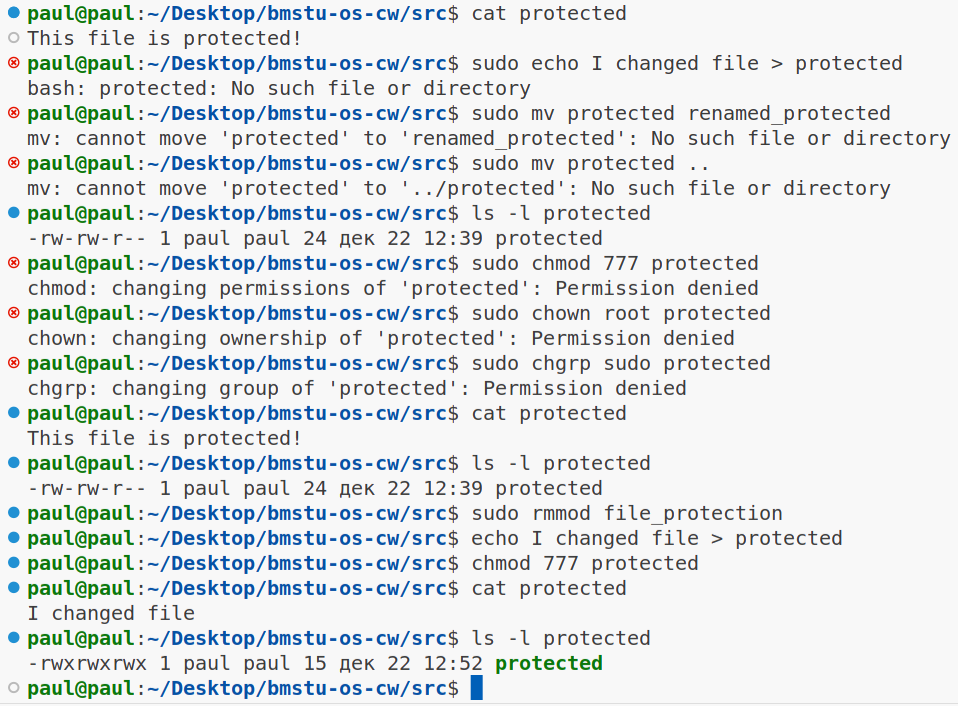
\includegraphics[width=152mm]{img/example.png}
	\caption{Демонстрация  работы  программы}
	\label{fig:example}
\end{figure}

\subsection*{Вывод}
В данном разделе были приведены примеры работы загружаемого модуля ядра и демонстрация защиты файла от описанных в аналитическом разделе действий.

Разработанная программа выполняет поставленную задачу: защищает файл от воздействия привилегированного пользователя, а именно от операций записи в файл, операций переименования, перемещения и удаления, а также операций изменения доступа к файлу, владельца файла и группы пользователей файла.




